\documentclass[fleqn,10pt]{wlscirep}
\usepackage[utf8]{inputenc}
\usepackage[T1]{fontenc}
\usepackage{siunitx}
\usepackage{xargs}  % Use more than one optional parameter in a new commands
\usepackage[colorinlistoftodos,prependcaption]{todonotes}

\sisetup{locale=US,group-minimum-digits=5,group-separator={,}}

\newcommandx{\alltodo}[2][1=]{\todo[author=Everyone,linecolor=red,backgroundcolor=red!25,bordercolor=red,#1]{#2}}
\newcommandx{\mctodo}[2][1=]{\todo[author=Matt,linecolor=blue,backgroundcolor=blue!25,bordercolor=blue,#1]{#2}}
\newcommandx{\comment}[2][1=]{\todo[author=Comment,linecolor=lime,backgroundcolor=lime!25,bordercolor=lime,#1]{#2}}
\newcommandx{\arhtodo}[2][1=]{\todo[author=Adam,linecolor=purple,backgroundcolor=purple!25,bordercolor=purple,#1]{#2}}

\title{A preprocessed open diffusion derivatives dataset from the Healthy Brain Network}

\author[1,*$\dagger$]{Adam Richie-Halford}
\author[2,$\dagger$]{Matthew Cieslak}
\author[4]{Lei Ai}
\author[5]{Sendy Caffarra}
\author[4]{Alexandre R. Franco}
\author[5]{Iliana Karipidis}
\author[3]{John Kruper}
\author[5]{Barbara Avelar Pereira}
\author[5]{Ethan Roy}
\author[2]{Valerie J. Sydnor}
\author[5]{Jason Yeatman}
\author[4]{Michael Milham}
\author[6]{Jul\_dugre}
\author[6]{amandamcgow}
\author[6]{SimonMB}
\author[6]{Nabbott}
\author[6]{AmjadSamara}
\author[6]{Shannon Grogans}
\author[6]{Zzzdeng}
\author[6]{HamidTurker}
\author[6]{Dragon}
\author[6]{Lshaffe6}
\author[6]{Hilarym}
\author[6]{faskybrain}
\author[6]{RaeYuan}
\author[6]{wanderinggrace}
\author[6]{sofie}
\author[6]{llotter}
\author[6]{valeriejill}
\author[6]{AkiNikolaidis}
\author[6]{Deagaric}
\author[6]{akoz}
\author[6]{summerf}
\author[6]{lindenmp}
\author[6]{mjl0062}
\author[6]{Nevena}
\author[6]{kat\_sh}
\author[6]{LeonF}
\author[6]{anjaue}
\author[6]{utooley1}
\author[6]{adrian\_neurosci}
\author[6]{mattwall}
\author[6]{Griffin SH}
\author[6]{jbourque}
\author[6]{averigiudicessi}
\author[6]{ncolenbi}
\author[6]{vtrip}
\author[6]{MeganHimes}
\author[6]{ti}
\author[6]{floundersmw}
\author[6]{itsyuchao}
\author[6]{jjfc}
\author[6]{Agwiesman}
\author[6]{bhaggerty}
\author[6]{benjamindeleener}
\author[6]{AnthonyJa}
\author[6]{seedyh}
\author[6]{nm\_fibr}
\author[6]{matthew2}
\author[6]{Li}
\author[6]{Gabriel Gonzalez-Escamilla}
\author[6]{Gianpaolo}
\author[6]{Mareike}
\author[6]{arielleered}
\author[6]{gdelap}
\author[6]{elliem}
\author[6]{skorenic}
\author[6]{Mark Wiesman}
\author[6]{SHKohl}
\author[6]{claudiap}
\author[6]{mackenzie}
\author[6]{jaewsong}
\author[6]{guillaume}
\author[6]{sadieneuro}
\author[6]{GuiomarNiso}
\author[6]{PSB}
\author[6]{elorenc}
\author[6]{smarek}
\author[6]{fsayed}
\author[6]{gthf61448}
\author[6]{WendyWang}
\author[6]{dcg2153}
\author[6]{mpeter55}
\author[6]{earoy}
\author[6]{cmich}
\author[6]{ikahhale}
\author[6]{czaj}
\author[6]{JodyFinch11}
\author[6]{albie}
\author[6]{holoships}
\author[6]{ckw84}
\author[6]{Gaga}
\author[6]{ecoffey}
\author[6]{jmayor}
\author[6]{jbryn}
\author[6]{jlurp20}
\author[6]{ShaoshiZ}
\author[6]{slhkam}
\author[6]{ckorponay}
\author[6]{BrunoHeblingVieira}
\author[6]{Yacine Mahdid}
\author[6]{harriet89}
\author[6]{Christian}
\author[6]{JonathanTSchneider}
\author[6]{bennewman}
\author[6]{sidchop}
\author[6]{Smeisler}
\author[6]{roryboyle}
\author[6]{cMadan}
\author[6]{MaryLena}
\author[6]{mkp}
\author[6]{Twelton}
\author[6]{dalez}
\author[6]{hyruuk}
\author[6]{ehhall}
\author[6]{jlhanson5}
\author[6]{smomara}
\author[6]{EvrenOzarslan}
\author[6]{ctw}
\author[6]{mollyr}
\author[6]{NChaku}
\author[6]{iliazaharov}
\author[6]{askeller}
\author[6]{clh64}
\author[6]{flat\_brainer}
\author[6]{H Farmer}
\author[6]{Jacobjcrouse}
\author[6]{Ryguy}
\author[6]{VincentBottom}
\author[6]{aomary}
\author[6]{aojha7}
\author[6]{wanderine}
\author[6]{Kahini}
\author[6]{bc1115}
\author[6]{adam}
\author[6]{sasims}
\author[6]{anovan}
\author[6]{patriciaschm}
\author[6]{dlsta}
\author[6]{berwe48}
\author[6]{Token Tech Chick}
\author[6]{Michael Cormican}
\author[6]{mhettwer}
\author[6]{pkirk}
\author[6]{lexlosia}
\author[6]{n00bmaster69}
\author[6]{Greki}
\author[6]{GuidoG}
\author[6]{ben}
\author[6]{yhahn1819}
\author[6]{GiuliaLiberati}
\author[6]{skyesinc}
\author[6]{djdlc85}
\author[6]{janderz8}
\author[6]{aiwiesman}
\author[6]{kurtzoner}
\author[6]{Dwin}
\author[6]{harman}
\author[2,$\ddagger$]{Theodore D. Satterthwaite}
\author[3,1,$\ddagger$]{Ariel Rokem}

\affil[1]{University of Washington, eScience Institute, Seattle, Washington, 98195, USA}
\affil[2]{University of Pennsylvania, Department of Psychiatry, Philadelphia, Pennsylvania, 19104, USA}
\affil[3]{University of Washington, Department of Psychology, Seattle, Washington, 98195, USA}
\affil[4]{Child Mind Institute, New York City, 10022, USA}
\affil[5]{Stanford University, Graduate School of Education and Division of Developmental and Behavioral Pediatrics, Stanford, California, 94305, USA}
\affil[6]{The Fibr Community Science Consortium}

\affil[*]{richford@uw.edu}
\affil[$\dagger$]{these authors contributed equally to this work}
\affil[$\ddagger$]{these authors contributed equally to this work}

%\keywords{Keyword1, Keyword2, Keyword3}

\begin{abstract}
\arhtodo[inline]{Write abstract}
\end{abstract}
\begin{document}

\flushbottom
\maketitle
\thispagestyle{empty}

\todo[inline]{%
    Note to reviewing authors:

    We use the \texttt{todonotes} package to keep track of remaining tasks and comments. You can add a task for Adam with the \texttt{\textbackslash{}arhtodo} command, a task for Matt with the \texttt{\textbackslash{}mctodo} command, a task for all reviewing authors with the \texttt{\textbackslash{}alltodo} command, and a general comment with the \texttt{\textbackslash{}comment} command.
}
\comment[inline]{Comments look like this.}
\arhtodo[inline]{Tasks for Adam look like this.}
\mctodo[inline]{Tasks for Matt look like this.}
\alltodo[inline]{Tasks for all reviewing authors look like this.}

\section*{Introduction}

The Healthy Brain Network (HBN) is a landmark pediatric mental health study
collecting MRI images and clinical assessment data from \num{10000} New York
City area children and adolescents \cite{alexander2017-yc}. The HBN dataset
contains a wealth of phenotypic and imaging data, including diffusion MRI (dMRI)
data, which allows for analysis of the physical properties of developing white
matter \cite{wandell2016-qt}. This dMRI data is openly available in raw form
through the Functional Connectomes Project and the International Neuroimaging
Data-Sharing Initiative (FCP-INDI), spurring collaboration on open big-data
reproducible science \cite{avesani2019-ey}. However, analysis of dMRI data must
start with a pipeline of critical preprocessing steps, such as eddy current
correction, motion correction, and adjustment of the gradient directions.
Because of the complexity of some of these steps, investigators may neglect to
perform preprocessing or may make errors that can induce bias in their
subsequent interpretation of the data \cite{jones2010-ps}. Furthermore, once
preprocessing is done correctly and transparently once, there is little need for
researchers to repeat this step. Thus, there is a need for an openly available
preprocessed diffusion derivative dataset that applies best practices in
preprocessing in a robust and transparent way \cite{cieslak2021-iq}.
Accordingly, here we introduce the HBN Preprocessed Open Diffusion Derivatives
(HBN-POD2), a large dataset for the analysis of structural brain connectivity
and pediatric mental health.

\section*{Results}

The aims of this study were fourfold
\begin{enumerate*}[%
    label=(\roman*),%
    before=\unskip{: },%
    itemjoin={{, }},%
    itemjoin*={{, and }}]
    \item curate the HBN MRI data into a fully-BIDS compliant MRI dataset
    \item perform state-of-the-art diffusion preprocessing using \emph{QSIPrep}
    \item assign QC scores to each subject using a combination of expert
    labelling, community science, and deep learning
    \item provide unrestricted public release of the outputs from each of these
    steps.
\end{enumerate*}

Figure \ref{fig:hbn-sankey} depicts the data provenance of the HBN-POD2 dataset.
Starting with MRI data from \num{2747} HBN participants available on FCP-INDI,
we curated these data for compliance with the Brain Imaging Data Structure
(BIDS) specification \cite{gorgolewski2016-lh} and preprocessed the structural
MRI (sMRI) and diffusion MRI (dMRI) data using \emph{QSIPrep}, resulting in
\num{2136} subjects with preprocessed, BIDS-compliant dMRI data.

\begin{figure}[ht]
    \centering
    % 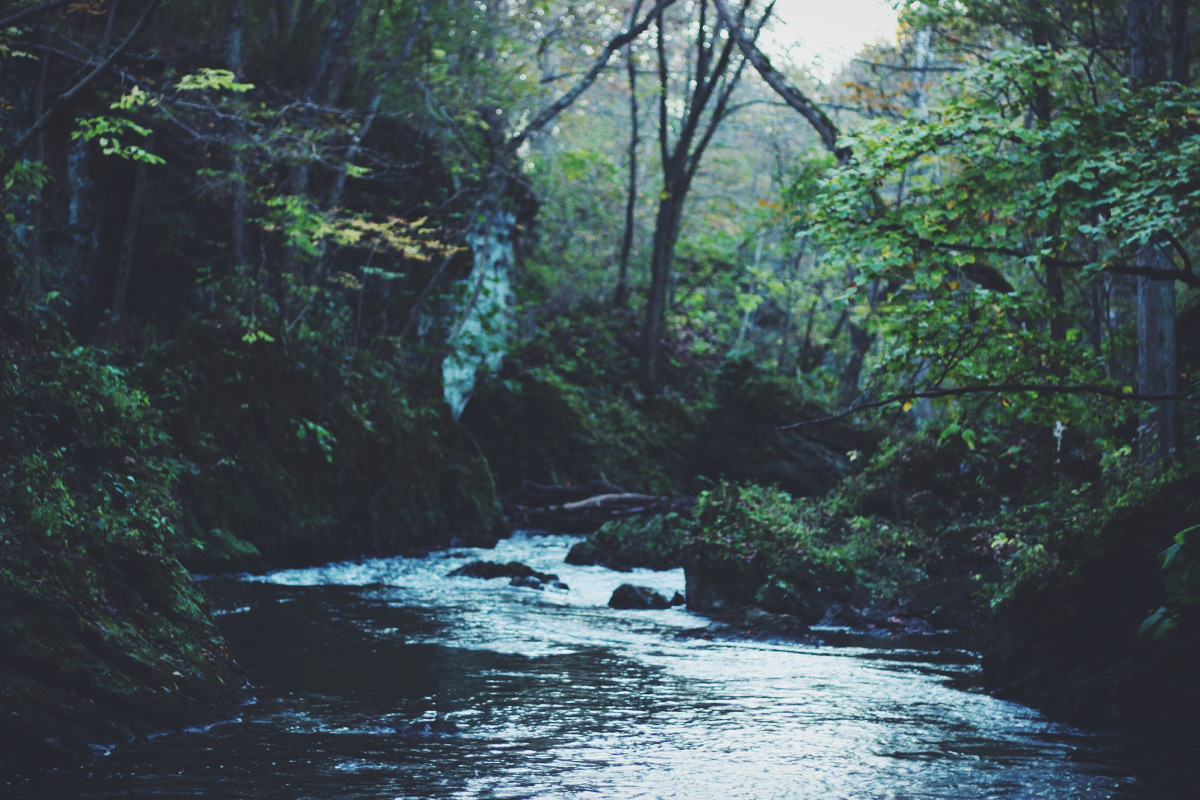
\includegraphics[width=\linewidth]{stream}
    \missingfigure{Insert sankey diagram}
    \caption{%
        {\bf HBN-POD2 data provenance}:
        Imaging data for \num{2747} subjects, aged 5-21 years and collected at four
        sites in the New York City area, was made available through the
        Functional Connectomes Project and the International Neuroimaging
        Data-Sharing Initiative (FCP-INDI).
        %
        These data were curated for compliance to the BIDS specification
        \cite{gorgolewski2016-lh} and availability of imaging metadata in json
        format. \num{2615} subjects met this specification.
        %
        Imaging data was preprocessed using \emph{QSIPrep} \cite{cieslak2021-iq}
        to group, distortion correct, motion correct, denoise, coregister and
        resample MRI scans. Of the BIDS curated subjects, \num{2136} subjects
        passed this step, with the majority of failures coming from subjects
        with missing dMRI scans.
        %
        Expert raters assigned QC scores to \num{200} of these participants,
        creating a ``gold standard'' QC subset. Community raters then assigned
        binary QC ratings to a superset of the gold standard containing
        \num{1653} participants. An image classification algorithm was trained
        on a combination of automated QC metrics from QSIPrep and community
        scientist reviews to ``extend'' the expert ratings to the community
        science subset.  Finally, a deep learning QC model was trained on the
        community science subset to assign QC scores to the entire dataset and
        to future releases from HBN.
        %
        The HBN-POD2 dataset, including QC ratings, is openly available through
        FCP-INDI.
    }
    \label{fig:hbn-sankey}
\end{figure}

\subsection*{Expert quality control}

- Qsiprep QC metric distributions and correlations with avg gold standard rating
- Two Scatterplots: y-axis is gold standard rating. X is either avg fibr rating or XGB output
- ROC curves for XGB models (add simple fibr average to that), add the CNN model
- Attribution masks from integrated gradients for select subjects (high consensus pass or fail)
- QC so what? Age prediction performance on QC strata after varying QC cutoff


\section*{Discussion}

We present HBN-POD2, one of the largest youth diffusion imaging datasets with
derived measures currently available. It is openly available and complies with
the current draft of the BIDS diffusion derivative specification. It will grow
continuously as the HBN study acquires more data, eventually reaching its
\num{10000} subject goal. The data is amenable to many different analyses,
including tractometry \cite{yeatman2012-rc}, graph theoretical analysis
\cite{yeh2020-nu}, and combinations with functional data for the same subjects.
The availability of standardized preprocessed diffusion data will allow
researchers to create and test hypotheses on the white matter properties
underlying behavior and disease, from reading and math acquisition to childhood
adversity and mental health. As such, this dataset will accelerate discovery at
the nexus of structural connectivity and neurodevelopmental and learning
disorders.

\section*{Methods}

Inputs for this study consisted of MRI data from the Healthy Brain Network
pediatric mental health study \cite{alexander2017-yc}, containing dMRI data from
\num{2747} subjects with ages 5-21. These data were measured using a
\qty{1.5}{\tesla} Siemens mobile scanner on Staten Island (SI) and three fixed
\qty{3}{\tesla} Siemens MRI scanners at sites in the New York area: Rutgers
University Brain Imaging Center (RUBIC), the CitiGroup Cornell Brain Imaging
Center (CBIC), and the City University of New York Advanced Science Research
Center (CUNY). Informed consent was obtained from each participant aged 18 or
older. For participants younger than 18, written consent was obtained from their
legal guardians and written assent was obtained from the participant. Voxel
resolution was \qtyproduct{1.8 x 1.8 x 1.8}{\mm} with \num{64} non-colinear
directions measured for each of $b=1000$ \unit{\second \per \mm^{2}} and
$b=2000$ \unit{\second \per \mm^{2}}.

\subsection*{BIDS curation}

We curated the imaging metadata for \num{2615} of the \num{2747} currently
available HBN subjects. Using dcm2bids and custom scripts, we conformed the data
to the Brain Imaging Data Structure (BIDS; \cite{gorgolewski2016-lh})
specification.  The BIDS-curated dataset is available on FCP-INDI and can be
accessed via AWS S3 at \url{s3://fcp-indi/data/Projects/HBN/BIDS_curated/}.

\mctodo[inline]{Add more BIDS curation information}

\subsection*{Preprocessing}

We performed dMRI preprocessing on \num{2136} subjects, using \emph{QSIPrep}
\cite{cieslak2021-iq} 0.12.1, which is based on \emph{Nipype} 1.5.1
\cite{nipype1,nipype2}, RRID:SCR\_002502. \emph{QSIPrep} a robust and scalable
pipeline to group, distortion correct, motion correct, denoise, coregister and
resample MRI scans.  In total, \num{417} subjects failed this preprocessing
step, largely due to missing dMRI files. In keeping with the BIDS specification,
the preprocessed dataset is available as a derivative dataset within the
BIDS-curated dataset and can be access on AWS S3 at
\url{s3://fcp-indi/data/Projects/HBN/BIDS_curated/derivatives/qsiprep/}.
\emph{QSIPrep} fosters reproducibility by automatically generating thorough
methods boilerplate for later use in scientific publications, which we use for
the remainder of this subsection to document each preprocessing step.

\begin{itemize}

\item {\it Anatomical data preprocessing}
The T1-weighted (T1w) image was corrected for intensity non-uniformity (INU)
using \texttt{N4BiasFieldCorrection} \cite{n4} (ANTs 2.3.1), and used as
T1w-reference throughout the workflow. The T1w-reference was then skull-stripped
using \texttt{antsBrainExtraction.sh} (ANTs 2.3.1), using OASIS as target
template. Spatial normalization to the ICBM 152 Nonlinear Asymmetrical template
version 2009c \cite{mni}, RRID:SCR\_008796 was performed through nonlinear
registration with \texttt{antsRegistration} \cite{ants}, ANTs 2.3.1,
RRID:SCR\_004757, using brain-extracted versions of both T1w volume and
template. Brain tissue segmentation of cerebrospinal fluid (CSF), white-matter
(WM) and gray-matter (GM) was performed on the brain-extracted T1w using
\texttt{FAST} \cite{fsl_fast}, FSL 6.0.3:b862cdd5, RRID:SCR\_002823.

\item {\it Diffusion data preprocessing}

Any images with a $b$-value less than \qty{100}{\second \per \mm^{2}} were treated
as a $b=0$ image. MP-PCA denoising as implemented in MRtrix3's
\texttt{dwidenoise}\cite{dwidenoise1} was applied with a 5-voxel window. After
MP-PCA, B1 field inhomogeneity was corrected using \texttt{dwibiascorrect} from
MRtrix3 with the N4 algorithm \cite{n4}.  After B1 bias correction, the mean
intensity of the DWI series was adjusted so all the mean intensity of the $b=0$
images matched across eachseparate DWI scanning sequence.

FSL (version 6.0.3:b862cdd5)'s eddy was used for head motion correction
and Eddy current correction \cite{anderssoneddy}. Eddy was configured
with a \(q\)-space smoothing factor of 10, a total of 5 iterations, and
1000 voxels used to estimate hyperparameters. A linear first level model
and a linear second level model were used to characterize Eddy
current-related spatial distortion. \(q\)-space coordinates were
forcefully assigned to shells. Field offset was attempted to be
separated from subject movement. Shells were aligned post-eddy. Eddy's
outlier replacement was run \cite{eddyrepol}. Data were grouped by
slice, only including values from slices determined to contain at least
\num{250} intracerebral voxels. Groups deviating by more than four standard
deviations from the prediction had their data replaced with imputed
values. Data was collected with reversed phase-encode blips, resulting
in pairs of images with distortions going in opposite directions. Here,
$b=0$ reference images with reversed phase encoding directions were used
along with an equal number of $b=0$ images extracted from the DWI scans.
From these pairs the susceptibility-induced off-resonance field was
estimated using a method similar to that described in \cite{topup}. The
fieldmaps were ultimately incorporated into the Eddy current and head
motion correction interpolation. Final interpolation was performed using
the \texttt{jac} method.

Several confounding time-series were calculated based on the
\emph{preprocessed DWI}: framewise displacement (FD) using the implementation
in \emph{Nipype} following the definitions by \cite{power_fd_dvars}. The DWI
time-series were resampled to ACPC, generating a \emph{preprocessed DWI run
in ACPC space}.

\item {\it MRtrix3 Reconstruction}

Reconstruction was performed using \emph{QSIprep} 0.12.1. Multi-tissue fiber
response functions were estimated using the dhollander algorithm. FODs were
estimated via constrained spherical deconvolution (CSD, \cite{originalcsd,
tournier2008csd}) using an unsupervised multi-tissue method
\cite{dhollander2019response, dhollander2016unsupervised}. Reconstruction was
done using MRtrix3 \cite{mrtrix3}. FODs were intensity-normalized using
mtnormalize \cite{mtnormalize}.

\end{itemize}

Many internal operations of \emph{QSIPrep} use \emph{Nilearn} 0.6.2
\cite{nilearn}, RRID:SCR\_001362 and \emph{DIPY} \cite{dipy}. For more details
of the pipeline, see
\href{https://qsiprep.readthedocs.io/en/latest/workflows.html}{the section
corresponding to workflows in \emph{QSIPrep}'s documentation}.

\subsection*{Cloud-based distributed preprocessing}

\arhtodo[inline]{Add information on cloudknot}
Using a previously developed cloud-computing library
\cite{richie-halford2018-kv} to parallelize the preprocessing over individual
subjects on spot instances in the Amazon Web Services Batch service, this dMRI
preprocessing cost less than \textdollar1.00 per subject.

\subsection*{Expert quality control}

The expert QC ``gold standard'' subset was created by randomly selecting 200
subjects from the preprocessed dataset, sampled such that the proportional site
distribution in the gold standard subset matched that of the preprocessed
dataset.

We created a web application for expert quality control of preprocessed dMRI,
called \emph{dmriprep-viewer} \cite{richie-halford2021-viewer}.
\comment[inline]{%
    We might change the name of the viewer now that it's going to be modality
    agnostic.%
}

\arhtodo[inline]{%
    Add information on dmriprep-viewer, the QC instruction video, and the expert QC
}

\subsection*{Community scientist quality control}

To assess image quality, we released a citizen science web application, drawing
on the success of a previous application in assessing the quality of HBN's
structural MRI data \cite{keshavan2019-er}. After a brief tutorial, citizen
scientists provided binary pass/fail ratings based on the
directionally-colorized fractional anisotropy from DTI of each subject's
preprocessed dMRI data. These citizen scientist ratings were then combined with
expert ratings to train a neural network to assign a quality control (QC) rating
to each subject.

\subsection*{Deep learning to predict quality control}

\begin{itemize}
    \item Fibr solution does not scale to new releases or left out data from this release.
    \item Solution deep learning
    \item Show architecture and point to the CT scan paper \cite{zunair2020-bs}.
    \item Two model types
    \item Data format (4-channels + QSIPrep QC metric input)
    \item Learning curves
    \item ROC AUC curves (move to results)
\end{itemize}

\subsection*{Brain age prediction}

\bibliography{hbn-pod2}

\section*{Acknowledgements}

We would like to thank Anisha Keshavan for useful discussions of community
science and web-based quality control. This manuscript was prepared using a
limited access dataset obtained from the Child Mind Institute Biobank, The
Healthy Brain Network dataset. This manuscript reflects the views of the authors
and does not necessarily reflect the opinions or views of the Child Mind
Institute.

\alltodo[inline]{Add grant numbers.}

\section*{Author contributions statement}

The first author named is the corresponding author. The last two authors named
share senior authorship. The first two authors named share lead authorship.  The
next ten authors' contributions extended beyond providing community science
annotations and are listed in alphabetical order. All other authors are Fibr
community scientists and are listed in descending order of the number of QC
labels they produced.

\alltodo[inline]{Please add your initials here as appropriate}

We describe contributions to the paper using the CRediT taxonomy \cite{brand2015-vd}:
\begin{itemize}
    \item Conceptualization: A.R-H., A.R., T.S., and M.C.;
    \item Methodology: A.R-H. and A.R.;
    \item Software: A.R-H. and M.C.;
    \item Validation: ;
    \item Formal Analysis: A.R-H. and M.C.;
    \item Investigation: A.R-H. and M.C.;
    \item Resources: M.M.;
    \item Data curation: M.C. and L.A.;
    \item Writing – Original Draft: A.R-H. and A.R.;
    \item Writing – Review \& Editing: ;
    \item Visualization: A.R-H.;
    \item Supervision: A.R. and T.S.;
    \item Project Administration: A.R-H. and A.R.;
    \item Funding Acquisition: A.R. and T.S.
\end{itemize}

\section*{Additional information}

To include, in this order: \textbf{Accession codes} (where applicable);
\textbf{Competing interests} (mandatory statement).

The corresponding author is responsible for submitting a
\href{http://www.nature.com/srep/policies/index.html#competing}{competing
interests statement} on behalf of all authors of the paper. This statement must
be included in the submitted article file.

\arhtodo[inline]{Add accession codes and competing interests statement.}

% \begin{figure}[ht]
% \centering
% 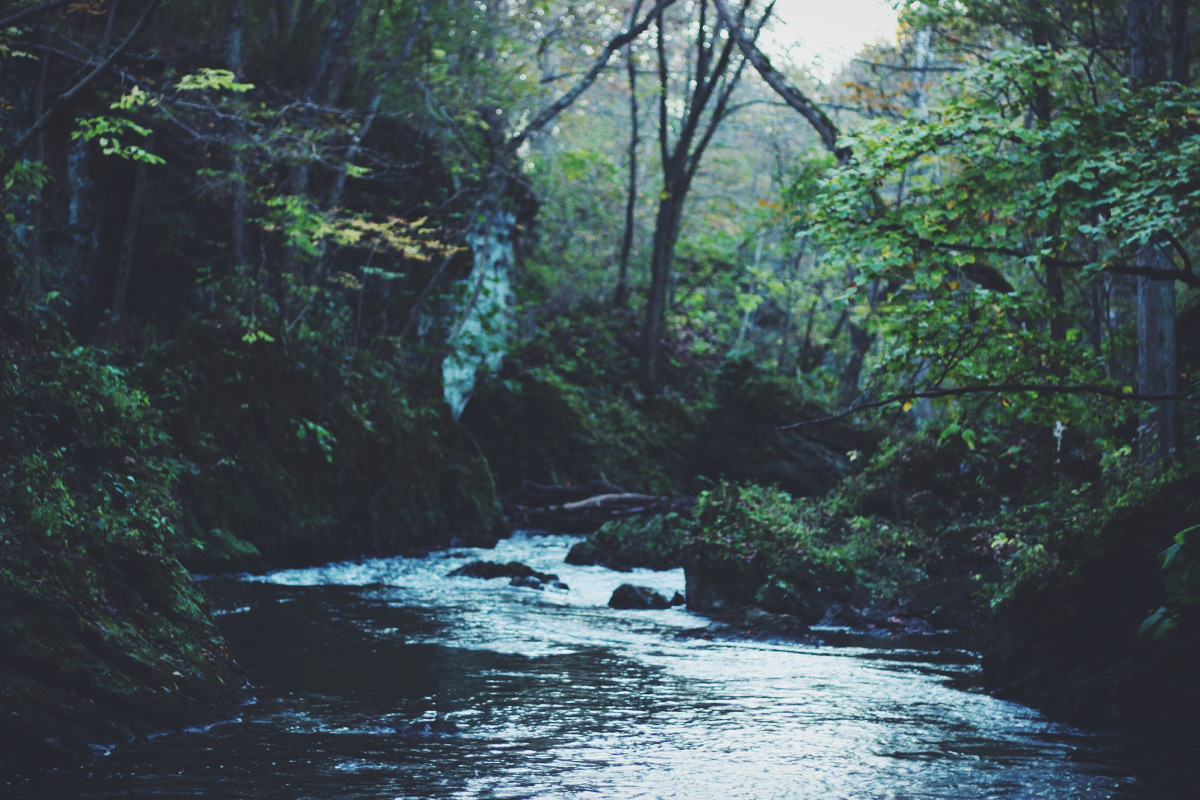
\includegraphics[width=\linewidth]{stream}
% \caption{Legend (350 words max). Example legend text.}
% \label{fig:stream}
% \end{figure}

% \begin{table}[ht]
% \centering
% \begin{tabular}{|l|l|l|}
% \hline
% Condition & n & p \\
% \hline
% A & 5 & 0.1 \\
% \hline
% B & 10 & 0.01 \\
% \hline
% \end{tabular}
% \caption{\label{tab:example}Legend (350 words max). Example legend text.}
% \end{table}

% Figures and tables can be referenced in LaTeX using the ref command, e.g. Figure \ref{fig:stream} and Table \ref{tab:example}.

\end{document}